\chapter{Graph Contraction and Connectivity}
\label{ch:graph-contraction}
\label{ch:gc}
{
\begin{notesonly}
\paragraph{Lecture 1: connectivity, graph theory, edge contraction.} 
\begin{enumerate}

\item
Draw graph that has edges between two
students if they agree (A lovers have an edge and B lovers have on
edge).  The graph will have two components, each of which is a
complete.  The complete graph will be too large for all students so
pick some vertices, you can use for example 3 vertices. You can pick
something that looks like the example graphs used for graphs in the
lecture notes.

\item Another graph to use is a person with their dog.  The vertices
  can be labeled ``human'' and ``dogpq'' where p and q are the paws.
  You can draw them as two  components and then draw a leash to
  connect them.  I did this and it was nice and funny.

\item Now, go over some definitions.
\begin{enumerate}

\item Subgraphs, vertex and edge induced.

\item Connectivity. 

\item Connected component.

\item Graph partitioning. 

\item Naming and partition map.
\end{enumerate}

\item Go back to the graphs for connected components.

\item Ask them for an algorithm to find the A and B lovers given
  this graph.  Discuss BFS and DFS based approaches.  Discuss the case
  where instead of just A and B, you have many components, where BFS
  will perform poorly.



\item 
Start the lecture with a game. Select a group of students that prefer
A over B and another group that prefers B over A.
%
A and B could be tea and coffee, dark or milk chocolate, creamy of
chunky peanut butter. 
%
Call about 20 students to the front of the lecture and ask them mix up
randomly as in a cocktail party.

%
Now ask each student to partner up with a student that has the same
preference.  Students can talk to anyone.
%
In graph theory, this is called a vertex matching.
%
Now, tell them to come together into two groups where one group
consists of students that prefer A over B and the other group consists
of students that prefer B over A. 
%
In graph theory this is called a connected component.  They have found
connected components in the graph.


\item Draw another graph where again you have edges as above but not
  all the edges, you can omit some edges.  For example, you can have
  each component such as a chain. Discuss BFS approach and talk about
  the problem.

\item Summary: you have introduced connectivity, discussed
  graph-search based solutions and why they don't work.  Now,
  presumably the students also did edge contraction and solved the
  connectivity problem.  So this is what we are going to build on.


\item Talk about techniques to solve the connectivity problem.  Divide
  and conquer. Why does it not work. Graph partitioning NP hard.

\item Contraction can work.  Allude to the fact that this is how the
  students solved the problem.  

\item Graph contraction design technique.

\item How to contract a graph? Compute vertex partitioning.  Pick a
  vertex to represent each partition.  Map to super-vertices.  Drop
  internal edges. Reroute cut edges.


\item We repeat, each graph contraction is called a round.

\item Based on how we select each partition, we have different
  algorithms. We will talk about edge partitioning now.


\item Edge partitioning.
\begin{enumerate}
\item Edge partitioning: each part consists of a single vertex or
  two vertices connected by an edge.

\item Edge contraction: graph contraction with edge partitioning. Use
  the circle example~\exref{gc::ep::circle}

\item How to select an edge partitioning?  \exref{gc::ec::matching}
  and show that this is not always easy.

  We can select a set of edges that do not share a vertex and then let
  the vertices not included be singletons.  The problem of finding
  such a set of edges is called the vertex matching problem: select a
  subset of edges such that no two edges.

  This can be turned into a game.  Perhaps introduce in the beginning.
  Ask the volunteer to partner someone (one and only one) in the group
  that matches their interest.


\item Maximal vertex matching. Can be solved requires too much
  work. We don't need a maximal one.

\item Puzzle: how to use a vertex matching this?

\item Greedy algorithm.  The problem with it.

\item Puzzle: how to find one in parallel?  We need to break the
  symmetry.  Can we use randomization?

\item There will likely be many suggestion.  We will analyze the
  algorithm where we flip a coin for each edge and select the edge if
  the edges incident on its end points all flip tails and the edge
  itself flips heads.

\item Analyze the algorithm on a circle

\item Can we improve the bounds?  Each vertex can select a neighbor,
  improves to n/4?
  Or each edge can flip a number between 1 and n and selects if it is
  the maximal. this would improve to n/3.

\item Does not work for many graph, talk about a star graph.


\end{enumerate}

\end{enumerate}


\paragraph{Lecture 2: star contraction.} 

\begin{enumerate}
\item Review:

\begin{enumerate}
\item Subgraphs, vertex induced, partitions, graph partitioning.
\item Connected components.
\item Graph contraction.  Idea: if small solve, otherwise partition
  the graph, and replace each part with a super-vertex, deleting
  internal but keeping cut edges.  Recur.

\item Graph contraction example: Draw example 16.4
\item Big question: how to partitong the graph
\item Edge partitioning and edge contraction. Idea: select a disjoins
  set of edges and contract them. Show
\item Draw example \exref{gc::ec::edge-contraction-example}
\item Describe the analysis on circles.  Describe why it fails on
  general graphs.
\end{enumerate}

\item Star graph.
\item Star partition.
\item Connectivity.
\item Analysis.

\end{enumerate}


\end{notesonly}



In earlier chapters, we have mostly covered techniques for solving
problems on graphs that were developed in the context of sequential
algorithms.  Some of them are easy to parallelize while others are
not.  For example, we saw that BFS has some parallelism since each
level can be explored in parallel, but there was no parallelism in
DFS.
%% Umut: this is unclear to me also sounds forced.  We are ok with 
%% sequential algorithms anyway.  We want to cover them.
%%
% \footnote{In
%   reality, there is parallelism in DFS when graphs are dense---in
%   particular, although vertices need to visited sequentially, with
%   some care, the edges
%   can be processed in parallel.}  
%%
There was limited parallelism in Dijkstra's algorithm, but there was
plenty of parallelism in the Bellman-Ford algorithm.
%
In this chapter we cover a technique called ``graph contraction''
that was specifically designed to be used in parallel algorithms and
that allows obtaining poly-logarithmic span for certain graph problems.

%% Not sure if this makes sense, because we make new graphs
%% instead of modifying them.
%%
% Also, so far, we have only described algorithms that do not modify
% a graph, but rather just traverse the graph, or update values
% associated with the vertices.  As part of graph contraction, in this
% chapter we will also study techniques that restructure graphs.   


\begin{notesonly}
  Please review the material on graphs (\secref{graph-theory}) before
  proceeding with the rest of this chapter, especially the sections on
  subgraphs and connectivity.
\end{notesonly}

%\section{Preliminaries}
Let's start with a definition of graph partition.
%
Recall that a partition of a set $A$ is a set $P$ of non-empty subsets
of $A$ such that each element of $A$ is in exactly one subset $B \in
P$; each susbet $B \in P$ is called a part or block.
%

\begin{definition}
Given a graph $G$, 
%
a \defn{graph partition} of $G$ is a collection of graphs 
%
$H_0 = (V_0, E_0), \ldots, H_{k-1} = (V_{k_1}, E_{k-1})$
%
such that 
%
% $\bigcup_{i=0}{V_i} =V$, $\forall i. 0 \le i,j < k, V_i \not= \emptyset$
% and  $i \not= j \implies V_i \cap V_j = \emptyset$, 
%
$\{V_0, \ldots, V_{k-1}\}$ is a set partition of $V$
and 
%
$H_0, \ldots, H_{k-1}$ 
%
are vertex-induced subgraphs of $G$ with respect to $V_0, \ldots, V_{k-1}$.
%
Each subgraph $H_i$ is called a part of $G$.
\end{definition}
%
In other words, a graph partition is a collection of graphs induced by
vertex-induced graphs of a  set partition of its vertices. 


In a graph partition, we can distinguish between two kinds of edges:
internal edges and cut edges. 
%
We call an edge $\{v_1,v_2\}$ an \defn{internal edge}, if $v_1\in V_i$
and $v_2 \in V_i$, and by construction $\{v_1,v_2\} \in E_i$.
%
We call an edge $\{v_1,v_2\}$ a \defn{cut edge}, if $v_1\in V_i$
and $v_2 \in V_j$  and $i \not= j$.
%
One way to partition a graph is to make each connected component a
block. In such a partition, there are no cut edges between the
partitions.

Sometimes it is useful to give a name or a label to each part in a
graph partition.  
%
A graph partition can then be described as a set of labels for the
parts and \defn{partition map} that maps each vertex to the label of
its part.  
%
The labels can be chosen arbitrarily but sometimes it is conceptually
and computationally easier to use a vertex inside a part as a name
(representative) for that part.
%


\begin{example}
\label{ex:preliminaries::partition1}
The partition 
%
$\cset{\cset{\vname{a},\vname{b},\vname{c}},\cset{\vname{d}},\cset{\vname{e},\vname{f}}}$
%
of the vertices
%
$\cset{\vname{a},\vname{b},\vname{c},\vname{d},\vname{e},\vname{f}}$, 
%
defines three parts as vertex-induced subgraphs.
\begin{center}
  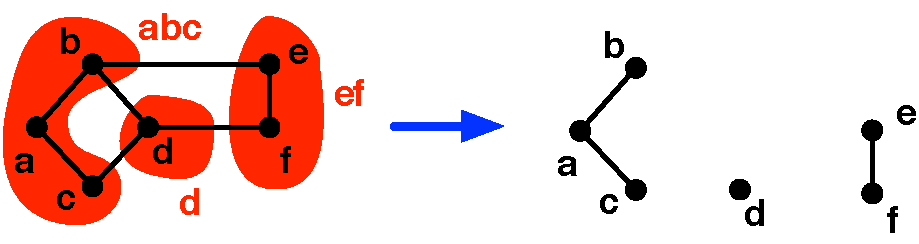
\includegraphics[width=4in]{preliminaries/contract-example8}
\end{center}
The edges $\cset{\vname{a},\vname{b}}$, $\cset{\vname{a},\vname{c}}$,
and $\cset{\vname{e},\vname{f}}$ are internal edges, and the edges
$\cset{\vname{c},\vname{d}}$, $\cset{\vname{b},\vname{d}}$,
$\cset{\vname{b},\vname{e}}$ and $\cset{\vname{d},\vname{f}}$ are
cut edges.

By labeling the parts ``\vname{abc}'', ``\vname{d}'' and
``\vname{ef}'', we can specify the graph partition with following partition map:
\\
%
$ (\cset{\vname{abc}, \vname{d}, \vname{ef}}, ~\cset{\vname{a} \mapsto
  \vname{abc}, \vname{b} \mapsto \vname{abc}, \vname{c} \mapsto
  \vname{abc}, \vname{d} \mapsto \vname{d}, \vname{e} \mapsto
  \vname{ef}, \vname{f} \mapsto \vname{ef}}).$

Instead of assigning a fresh label to each part, we can choose a
representative vertex.
%
For example, by picking $\vname{a}, \vname{d}$, and $\vname{c}$ as
representatives, we can represent the partition above using the
following partition map
\[
(\cset{\vname{a},\vname{d},\vname{e}}, 
 \cset{\vname{a} \mapsto \vname{a}, \vname{b} \mapsto \vname{a}, 
       \vname{c} \mapsto \vname{a}, \vname{d} \mapsto \vname{d}, 
       \vname{e} \mapsto \vname{e}, \vname{f} \mapsto \vname{e}}).
\]

\end{example}

\section{Graph Contraction}

Graph contraction is a technique for computing properties of graphs in
parallel.  As a contraction technique, it is used to solve a problem
instance by reducing it to a smaller instance of the same problem.
%
\begin{question}
Can we solve graph problems using divide-and-conquer? 
\end{question}
%
Graph contraction is important, since divide-and-conquer
can be difficult to apply in graph problems efficiently.  This is
because divide and conquer usually requires partitioning graphs into smaller
graphs in a balanced fashion such that the number of cut edges is
minimized.  Since graphs can be highly irregular, however, they can be
difficult to partition. In fact, graph partitioning problems are typically NP-hard.
%
The rest of this section describes the graph-contraction design
technique and two approaches to graph-contraction: edge contraction
and star contraction.

The key idea behind graph contraction is to contract the input graph
to a smaller \defn{quotient graph}, solve the problem on the quotient
graph, and then use that solution to construct the solution for the
input graph.  
%
We can specify this technique as an inductive algorithm-design
technique (\dtref{gc::gc-technique}) as follows.


\begin{designtechnique}[Graph Contraction]~
\label{dt:gc::gc-technique}
\begin{description}
\item[Base case:] If the graph is small (e.g., it has no edges), then compute
  the desired result.
\item[Inductive case:]~
\begin{itemize}
\item Contract the graph into a smaller quotient graph.
\begin{itemize}
\item Partition the graph into parts.
\item Contract each part to a single super-vertex.
\item Drop internal edges.
\item Reroute cut edges to corresponding super-vertices.  
\end{itemize}

\item Recursively solve the problem for the quotient graph.
\item Using the result for the quotient graph, compute the result
  for the input graph.
\end{itemize}
\end{description}
\end{designtechnique}


% \begin{simpleexample} [An example graph contraction]

%   An illustration of how we wish to apply graph contraction to solve
%   the connectivity problem.  In order to solve the problem, as we
%   contract the graph, we do not alter the connectivity of the
%   vertices: vertices that are not connected should not become
%   connected and vice versa.

% \begin{center}
% 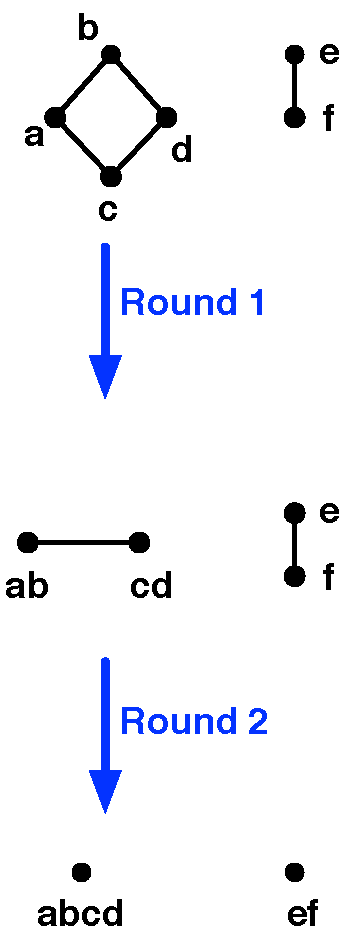
\includegraphics[width=1.5in]{graph-contraction/contraction-example}
% \end{center}
% \end{simpleexample}

The key step of graph contraction is the construction of the quotient.
%
To this end, we partition the graph and construct a quotient
graph, where each part in the partition is represented by a
vertex in the quotient graph.
%
We can construct the quotient graph by creating a
\defn{super-vertex} for each partition
%
We then consider each edge $(u,v)$ in the graph.  If the edge is an internal
edge, then we skip it.
%
Otherwise,  we create a new edge between the
super-vertices representing the parts containing $u$ and $v$.
%
Since there can be many
cut edges between two parts, we may create multiple edges between
two super-vertices.  We can remove such edges or leave them in the graph, in
which case we would be working with multigraphs.  In this chapter, we
shall remove duplicate edges, because this is simpler for our
purposes.
%
The process of identifying a partition and updating the edges is
called a \defn{round of graph contraction}. 
%
In a graph contraction, rounds are repeated until there are no edges
left.


An important property of graph contraction is that it is guided by a graph partition.  Since parts in a graph partition are disjoint, each vertex in the graph is mapped to one unique vertex in the quotient graph.

\begin{example}
\label{ex:gc::contract-example}

One round of graph contraction:
\begin{center}
  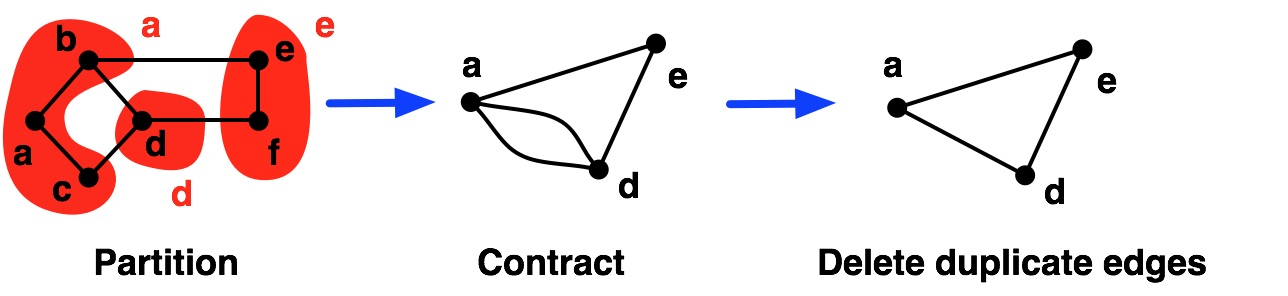
\includegraphics[width=5.7in]{graph-contraction/contract-example5}
\end{center}

Contracting a graph down to a single vertex in three rounds:
\begin{center}
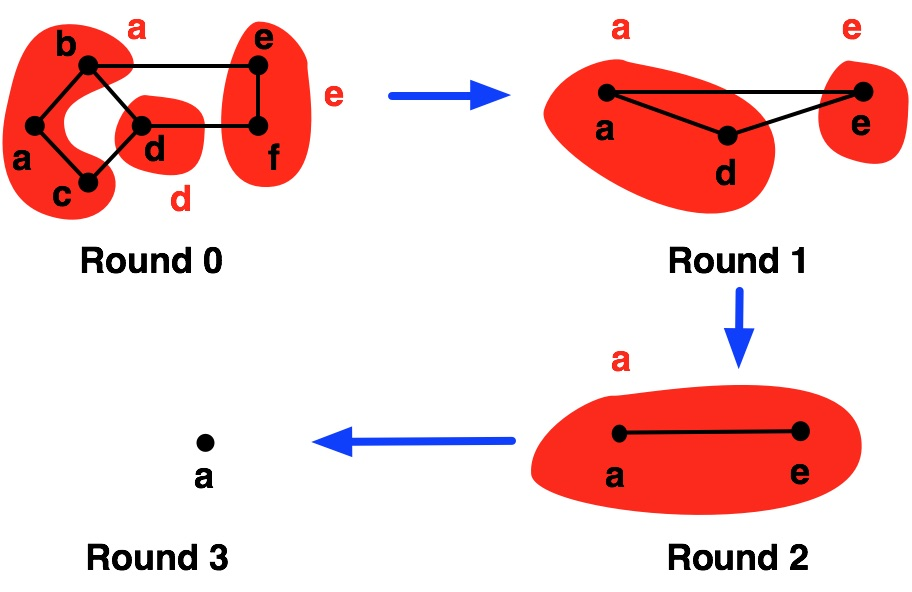
\includegraphics[width=4.0in]{graph-contraction/graph-contraction-example-1}
\end{center}
\end{example}

As described, the graph-contraction technique is generic in the kind
of graph partition used for constructing the quotient graph.  In the
rest of this chapter, we will consider two techniques, edge
partitioning and star partitioning, and the resulting
graph-contraction algorithms.


\subsection{Edge Partition and Edge Contraction}
\label{sec:gc::edge-partition}

Edge partitioning is a graph-partitioning technique.  In an \defn{edge
  partition},  each part is either a single vertex or two vertices
connected by an edge.  We use the term \defn{edge  contraction} to
refer to a graph contraction performed by using edge partitions.



\begin{example}
\label{ex:gc::ep::circle}
An example edge partition in which every part consists of two
vertices and an edge between them.  Contracting the graph based on
this partition yields a quotient graph with half as many vertices
and edges.
\begin{center}
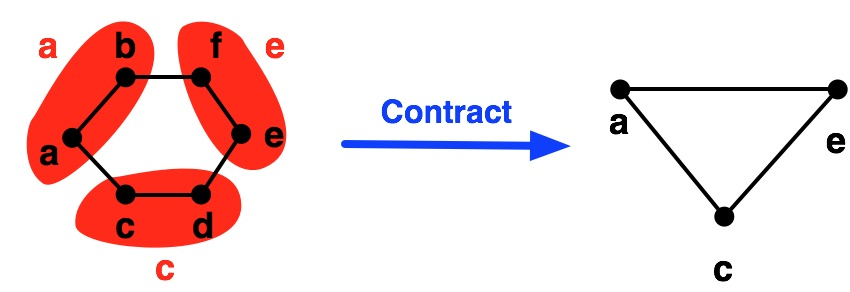
\includegraphics[scale=.65]{graph-contraction/edge-contraction-example-1}
\end{center}

Note that in general, parts cannot be just pairs of vertices, because
the graph might not have an even number of vertices, but even if it
does (no pun intended), it is likely that it cannot be partitioned
into a set of pairs joined by edges.
\end{example}

%
\begin{question}
How can we construct an edge-partitioning in the general case?
\end{question}
%
We can construct an edge partition by selecting an \defn{independent
  edge set}, or \defn{vertex matching},
where no two edges share a vertex, and placing all the
remaining vertices that are not incident an a selected edges into singleton
sets.
%
The problem of
finding a vertex matching is called the \defn{vertex-matching
  problem}.

\begin{definition} 
A \defn{vertex matching} for an undirected graph $G = (V,E)$
is a subset of edges $M \subseteq E$ such that no two edges in $M$
share a vertex.  
\end{definition}

\begin{example}
\label{ex:gc::ec::matching}
A vertex matching for our favorite graph (highlighted edges) and the
corresponding parts.
\begin{center}
  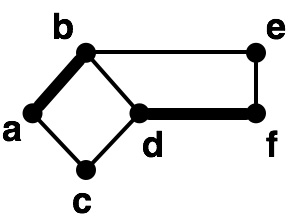
\includegraphics[width=1.5in]{graph-contraction/matching-example}
\hspace{1in}
  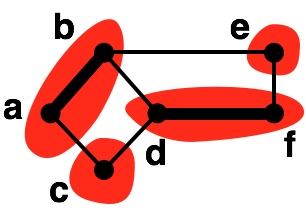
\includegraphics[width=1.5in]{graph-contraction/matching-example-partitioned}
\end{center}
The vertex matching defines four parts (circled), two of them defined
by the edges in the matching, $\cset{\vname{a},\vname{b}}$ and
$\cset{\vname{d},\vname{f}}$, and two of them are the unmatched
vertices \vname{c} and \vname{e}.
\end{example}


The problem of finding the largest vertex matching for a graph is
called the \defn{maximum vertex matching} problem.  Many algorithms
for this  well-studied problem have been proposed, including one that can solve the problem in
  $O(\sqrt{|V|}|E|)$ work.  For graph contraction, we do not need a
  maximum matching but one that it is sufficiently large.
%
\begin{question}
Describe an algorithm for finding a vertex matching.
\end{question}
%
For example, 
we can use a greedy algorithm to construct a vertex matching by going
through the edges one by one maintaining an initially empty set $M$
and for each edge, if no edge in $M$ is already incident on its
endpoints then add it to $M$, otherwise toss it.  The problem with
this approach is that it is sequential since each decision depends on
previous decisions.
%
\begin{question}
Describe a parallel algorithm for  vertex matching?
\end{question}
%
To find the vertex matching in parallel, we will need to make local
decisions at each vertex.  One possibility is for each vertex to
select one of its neighbors to match with.
%
Such a selection can be done in parallel but 
%
\begin{question}
What is the problem with this approach? 
\end{question}
%
there is one problem:  multiple vertices might select
the same vertex to match with.  
%
We therefore need a way
to {\em break the symmetry} that arises when two vertices try to match with the same vertex.
%
\begin{question}
Can you use randomization to break the symmetry? 
\end{question}
%
We can use randomization to break the symmetry.   For example,
we can  flip a coin for each
edge $(u,v)$ in parallel and 
select the edge, effectively matching $u$ and $v$,  if the coin
for the edge comes up heads and all the edges incident on
$u$ and $v$ flip tails.  This guarantees that a vertex is matched with
at most one other vertex.

\begin{example}[Edge contraction]
\label{ex:gc::edge-contract-example}

An example edge contraction illustrated.

\begin{center}
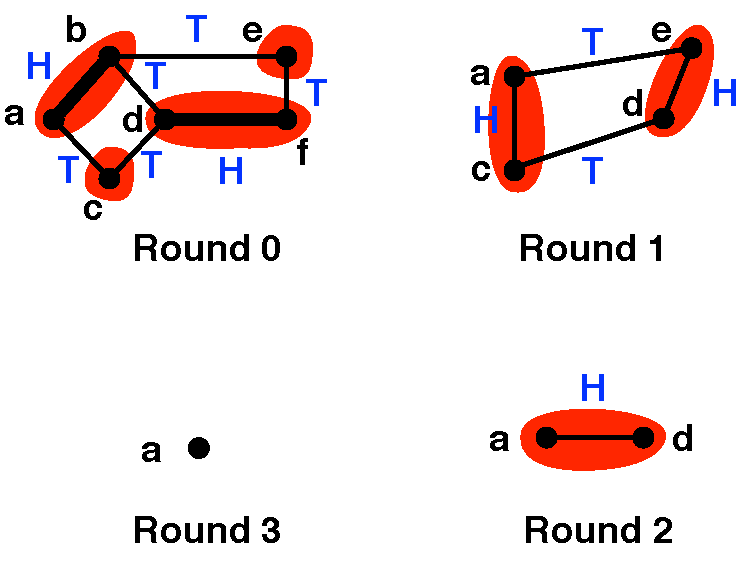
\includegraphics[width=3.5in]{graph-contraction/edge-contraction-example}
\end{center}

\end{example}


Let us analyze how effective this
approach is in selecting a reasonably large matching.  We first
consider cycle graphs, consisting of a single cycle and no other
edges.  In such a graph every vertex has exactly two neighbors.
\begin{example}
A graph consisting of a single cycle.    
  \begin{center}
  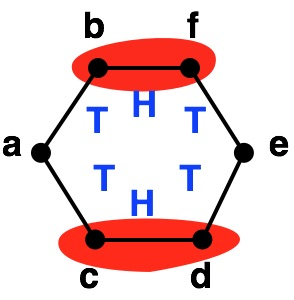
\includegraphics[scale=.65]{graph-contraction/cycle-graph}
  \end{center}
Each edge flips a coin that 
comes up either heads ($H$) or tails ($T$).    We select an edge if it 
turns up heads and all other edges incident on its endpoints are 
tails.    In the example  the edges $\cset{\vname{c},\vname{d}}$
and $\cset{\vname{b},\vname{f}}$
are selected.
 \end{example}
We want to
determine the probability that an edge is selected in such a graph.
Since the coins
are flipped independently at random, and each vertex has degree two, the probability that an edge
picks heads and its two adjacent edges pick tails is $\frac{1}{2}
\cdot \frac{1}{2} \cdot \frac{1}{2} = \frac{1}{8}$.   To
analyze the number of  edges  selected in expectation,   let $R_e$ be an
indicator random variable denoting whether $e$ is selected or not,
that is $R_e = 1$ if $e$ is selected and $0$ otherwise.  Recall that
the expectation of indicator random variables is the same as the
probability it has value $1$ (true).  Therefore we have $E[R_e] =
1/8$.
%
Thus summing over all edges, we conclude that expected number of edges
deleted is $\frac{m}{8}$ (note, $m=n$ in a cycle graph). 

\begin{todo}
We need to state this as a theorem.  It is not quite stated in this way.
\end{todo}

In the chapter on randomized algorithms \secref{kthsmallest} we argued
that if each round of an algorithm reduces the size by a constant
fraction in expectation, and if the random choices in the rounds are
independent, then the algorithm will finish in $O(\log n)$ rounds with
high probability.  Recall that all we needed to do is multiply the
expected fraction that remain across rounds and then use Markov's
inequality to show that after some $k \log n$ rounds the probability
that the problem size is a least 1 is very small.  For a cycle graph,
this technique leads to an algorithm for graph contraction with linear
work and $O(\log^2{n})$ span---left as an exercise.

\begin{question}
  Can you think of a way to improve the expected number of edges
  deleted?
\end{question}

There are several ways to improve the number of deleted edges.  One
way is for each vertex to pick one of its neighbors and to select an
edge $(u,v)$ if it was picked by both $u$ and $v$.  In the case of a
circle, this increases the expected number of deleted edges to
$\frac{m}{4}$. 
%
Another way is let each edge pick a random number in some range and
then select and edge if it is the local maximum, i.e., it picked the
highest number among all the edges incident on its end points. This
increases the expected number of edges contracted in a circle to
$\frac{m}{3}$.

Although edge contraction works quite well with cycle graphs, or
sequentially with the appropriate data structures, it does not 
work well for arbitrary graphs.  The problem is in edge contraction, only one edge incident on a vertex can be
contracted in each round.  Therefore vertices with high degrees, will
have to contract their neighbors one at a time.  The example below
illustrates a particularly difficult graph, called a star graph, for
edge contraction.
%
\begin{example}
\label{ex:gc::star}
A star graph with center $v$ and eight satellites.
  \begin{center}
  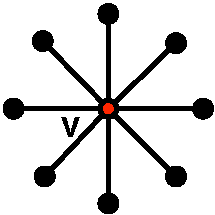
\includegraphics[scale=.75]{graph-contraction/star-graph1}
  \end{center}
\end{example}


More precisely, we can define a star graph as follows.
\begin{definition}[Star Graph]
  A \defn{star} graph $G = (V,E)$ is an undirected graph with a
  \defn{center} vertex $v \in V$, and a set of edges $E$ that attach
  $v$ directly to the rest of the vertices, called
  \defn{satellites}, i.e. $E = \cset{\cset{v,u} : u
    \in V \setminus \cset{v}}$.
\end{definition}
Note that a single vertex and a single edge are both star graphs.


It is not difficult to convince ourselves that on a star graph with
$n$ vertices---$1$ center and $n-1$ satellites---any edge partitioning
algorithm will take $\Omega(n)$ rounds.  To fix this problem we need
to be able to form parts that consist of more than just edges.

\begin{todo}
I (Umut) find the remark below quite confusing. 
\end{todo}

\begin{remark}
  An abstract data type called disjoint sets is often used to contract
  graphs sequentially.  Disjoint sets supply two functions:
  \defn{union}, which joins two components, and \defn{find}, which
  finds what component a vertex is in.  In our framework, the union
  operation is simply edge contraction across a single edge, and the
  find is just a lookup in the partition map.  Semantically for a
  partition map $P$ we can define \cname{union} as:

\begin{lstlisting}[numbers=none]
  union$(P,u,v)$ = $\{u' \mapsto $ if $(v' = u)$ then $v$ else $v'$ 
                 : $(u' \mapsto v') \in P\}$
\end{lstlisting}
where here we have made $v$ the new representative of the super-vertex
$\cset{u,v}$, and have updated all vertices that used to point to $u$
to now point to $v$.
Implementing the \cname{union} this way, however, is inefficient since
it can require updating a lot of vertices.  It turns out that the
operations can be can be implemented much more efficiently.  Indeed
one can implement a data structure that only requires amortized
$O(\alpha(n))$ work per operation, where $\alpha(n)$ (the inverse
Ackermann function) is a function that is very close ot $O(1)$, and
$n$ is the number of operations.
\end{remark}


\subsection{Star Partition and Star Contraction}
\label{sec:gc::star-partitioning}

In an edge partition, if there is an edge incident on a vertex~$v$ is
selected as a part, then none of the other edges incident on $v$ can be their own
part. This limits the effectiveness of edge partitioning, because it
is unable to contract significantly graphs with high-degree vertices.
%
In this section, we describe an alternative technique: star
partition.  

In \defn{star partitioning}, we partition a graph $G$ by selecting
parts of $G$ to correspond to subgraphs of $G$ that are stars.  For
example in \exref{gc::star}, the whole graph can be selected as a
single partition.  We refer to a graph contraction where parts
are selected by star partitioning a \defn{star contraction}.

\begin{example}
  In the graph shown below on the left, we first find two disjoint stars. We
  then partition the graph into two parts, each defined as the
  vertex-induced subgraphs of the two stars.

\begin{center}
\small
\begin{tabular}{lll}
\multicolumn{3}{c}{
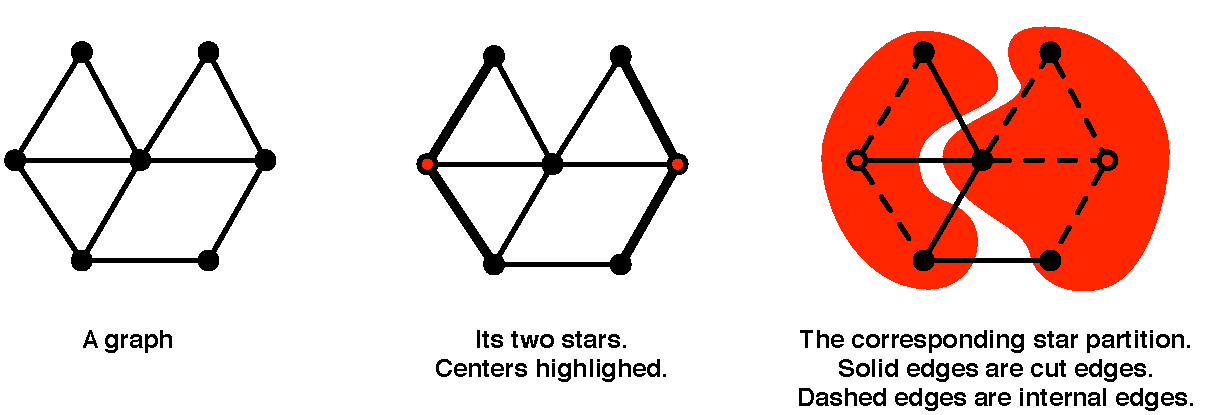
\includegraphics[width=0.9\textwidth]{graph-contraction/star-decomposition-1}
}
% \\
% A graph.\hspace{1in} & Two two stars,\hspace{1in} & The corresponding star partition.
% \\
% & Centers highlighted. & Solid edges are cut edges. 
% \\
% & & Dashed edges are internal edges. 
\end{tabular}
\label{ex:gc::star}
\end{center}
\end{example}



\begin{question}
How can we star-partition a graph? 
\end{question} 

As with edge partitions, it is possible to construct star partitions
sequentially.  One approach proceeds by adding start incrementally:  start with an arbitrary vertex $v$ and make $v$ the center
of a star; then, attach as satellites all the unattached neighbors of
$v$;  remove now $v$ and its satellites from the graph, and
recursively repeat the same process with the remaining graph.
%
Note that a vertex is the simplest form of a star.  
%
So if we have isolated vertices remaining, each will form a
\defn{singleton star} consisting of a single vertex.

\begin{question}
How can we star partition a graph in parallel? 
\end{question} 
%
We can also construct star partitions in parallel by making local
independent decisions at each vertex.  As in edge partitioning, we can
use randomization to break symmetry.
%
\begin{question}
Can you think of a randomized approach for selecting stars?
\end{question}
%
One approach proceeds as follows. 
%
Flip a coin for each vertex.
%
If a vertex flips heads, then it becomes the center of a star. 
%
If a vertex flips tails, then it attempts to become a satellite by
finding a neighbor that is a center. 
%
If no such neighbor exists (all neighbors have flipped tails or the
vertex is isolated), then the vertex becomes a center.
%
If a vertex has multiple centers as neighbors, it can pick one
arbitrarily.
%
\begin{question}
Is this algorithm guaranteed to create the smallest number of stars?
\end{question}
%
This approach might not be optimal in the sense that it might not create
the smallest number of stars but, as we shall see, this is acceptable
for our purposes, because we  only need to reduce the size
of the graph by a constant factor.  

\begin{example} 
\label{ex:startpartition}
An example star partition. Vertices $\vname{a}$ and $\vname{b}$, which
flip heads, become centers. Vertices $\vname{c}$ and $\vname{e}$,
which flipped tails, attempt to become satellites by finding a center
among their neighbors, breaking ties arbitrarily. 
%
If  a vertex does not have a neighbor that flipped heads, then it becomes a singleton star (e.g., vertex $d$).
%
We end up with three stars: the star with center $\vname{a}$ (with no
satellites), the star with center $\vname{b}$ (with two satellites),
and the singleton star $\vname{d}$.
%
The star partition thus yields  three parts, which
consists of the subgraphs  induced by each star.

\begin{center}
  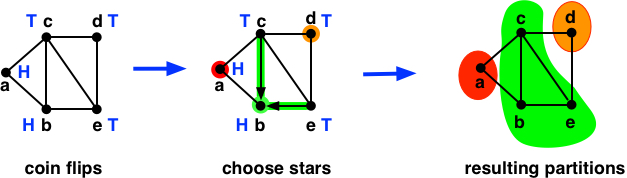
\includegraphics[width=5in]{graph-contraction/star-find0}
\end{center}

\end{example}


\newcommand{\cheads}{\cname{heads}}

To specify the star-partition algorithm, we need
a source of randomness.
%
For this, 
we assume that each vertex is given a (potentially infinite) sequence
of random and independent coin flips. The $i^{th}$ element of the
sequence can be accessed via the function
\[
\cheads(v,i) : V \times \mathbb{Z} \to \mathbb{B}, 
\]
which returns \cd{true} if the $i^{th}$ flip on vertex $v$ is heads
and false otherwise. Since most machines don't have true sources of
randomness, in practice this can be implemented with a pseudorandom
number generator or even with a good hash function. 

\begin{figure}
%require an undirected graph $G=(V,E)$ and round number $i$
%return $V'$ = remaining vertices after contraction,
%          $P$ = mapping from $V$ to $V'$
\begin{algorithm}[Star Partition]~
\label{alg:gc::starPartition}
\begin{lstlisting}[numbers=left]
starPartition $(G=(V,E),i)$ =
let
  (* Find the arcs from satellites to centers *)
  $\mathit{TH}$ = $\csetf{(u,v) \in E}{\neg \cheads(u,i) \land \cheads(v,i)}$ @\label{line:flip}\vspace{.1in}@
  (* Partition map from satellites to centers *)
  $P$ = $\bigcup_{(u,v) \in \mathit{TH}} \cset{u \mapsto v}$ @\vspace{.1in}\label{line:starmerge}@
  (* Super vertices are centers and unmatched ones *)
  $V'$ = $V \setminus \cname{domain}(P)$@\vspace{.1in}@
  (* Map super-vertices to themselves *)
  $P'$ = $\cset{u \mapsto u : u \in V'}$ @\label{line:self}\vspace{.1in}@
in $(V', P' \cup P)$ end
\end{lstlisting}
\end{algorithm}
\end{figure}

\algref{gc::starPartition} illustrates the code for star
partitioning.  
%
The function \ttt{starPartition} takes as argument a graph and a round
number, and returns graph partition specified by a set of centers and
a partition map from all vertices to centers.
%
The algorithm starts by flipping a coin for each vertex and selecting the directed
edges that point from tails to heads---this gives
the set of edges $\mathit{TH}$.
%
In this set of edges, there can be multiple edges from the same
non-center. Since we want to choose one center for each satellite, we
remove duplicates in \lineref{starmerge}, by creating a set of
singleton tables and merging them. 
%
More specifically, the union is shorthand for the code
\begin{quote}
\begin{lstlisting}[numbers=none]
Set.reduce (Table.union (fn (x,y) => x)) $\emptyset$ $\cset{\cset{u \mapsto v} : (u,v) \in \mathit{TH}}$.
\end{lstlisting}
\end{quote}
%
This completes the selection of satellites and their centers. 
%
The algorithm next determines the set of super vertices, which
can become the vertices of the quotient graph in contraction, as all
the vertices minus the satellites.
%
To complete the process, the algorithm determines each super vertex 
and matches it with itself (\lineref{self}).
%
This effectively promotes unmatched non-centers to centers, forming
singleton stars, and matches all centers with themselves.  
%
Finally, the algorithm constructs the partition map by  uniting the
mapping for the satellites and the centers.

\begin{example}
The  star-partition algorithm proceeds on the graph in
\exref{startpartition} as follows.
%
First, it computes
%
\[
\mathit{TH} =
\cset{(\vname{c},\vname{a}),(\vname{c},\vname{b}),(\vname{e},\vname{b})},
\]
%
as the edges from satellites to centers.  
%
Now, it
converts each edge into a singleton table, and merges all the tables into the
table, which is going to become part of the partition map:
%
\[
P = \cset{\vname{c} \mapsto \vname{b},\vname{e} \mapsto \vname{b}}.
\]
%
Note that the edge $(\vname{c},\vname{a})$ has been removed since when
uniting the tables, we selects only one element for each key in the
domain.  
%
Now for all remaining vertices
%
$V' = V \setminus \cname{domain}(P) = \cset{\vname{a},\vname{b},\vname{d}}$
we map them to themselves, giving:
%
\[
P' = \cset{\vname{a} \mapsto \vname{a}, \vname{b} \mapsto \vname{b},
  \vname{d} \mapsto \vname{d}}.
\]
%
The vertices in $P'$ are the centers.
%
Finally we merge $P$ and $P'$ to give to construct the partition map
%
\[
P' \cup P = \cset{\vname{a} \mapsto \vname{a}, \vname{b} \mapsto \vname{b}, \vname{c} \mapsto \vname{b}, \vname{d} \mapsto
    \vname{d}, \vname{e} \mapsto \vname{b}}.
\]
\end{example}

\newcommand{\nn}{\ensuremath{n_\bullet}}

\paragraph{Analysis of Star Partitioning.}  

By examining the algorithm, we can conclude the following work and
span bounds for the star partitioning algorithm.

\begin{todo}
This theorem needs a proof.  What is the graph representation? 
It seems like it is an edge set representation.

The big union would require logn span do we need inject here?

\end{todo}

\begin{theorem}[Star Partitioning]
Based on the array-based cost specification for sequences and
single-threaded sequences, the cost of \cname{starPartition} is $O(n +
m)$ work and $O(\log n)$ span for a graph with $n$ vertices and $m$
edges.
\end{theorem}


Let's also bound the number of satellites found by
\cname{starPartition}.
%
Note first that there is a one-to-one mapping between the satellites
and the set $P$ computed by  the algorithm.
%
\begin{question}
 In expectation, how big is $P$?  
\end{question}
%
The following lemma shows that on a graph with $\nn$~non-isolated
vertices, the size of~$P$ and thus the number of satellites is at least
$\nn/4$ in expectation.

\begin{lemma}
  For a graph $G$ with $\nn$ non-isolated vertices, the expected
  number of satellites in a call to \cname{starPartition}~$(G,r)$ with
  any~$r$ is at least $\nn/4$.
\end{lemma}

\begin{proof}
  For any vertex $v$, let $H_v$ be the event that a vertex $v$ comes
  up heads, $T_v$ that it comes up tails, and $R_v$ that $v \in
  \cname{domain}(P)$ (i.e, it is a satellite).
%
  Consider any non-isolated vertex $v \in V(G)$.  By definition, we
  know that a non-isolated vertex $v$ has at least one neighbor $u$.
  So, we know that $T_v \land H_u$ implies $R_v$, since if $v$ is a
  tail and $u$ is a head $v$ must either join $u$'s star or some other
  star.  Therefore, $\prob{R_v} \geq \prob{T_v} \prob{H_u} = 1/4$.  By
  the linearity of expectation,  the expected number of satellites is
  \begin{align*}
    \expct{\sum_{v: v \text{ non-isolated}} \onef{R_v}} & = \sum_{v: v
      \text{ non-isolated}} \expct{\onef{R_v}} 
\\[2mm]
  & \geq \nn/4.
  \end{align*}
  The final inequality follows because we have $\nn$ non-isolated
  vertices and because the expectation of an indicator random variable
  is equal to the probability that it takes the value $1$.
\end{proof}

\begin{notesonly}
Consider the random variable that a vertex becomes a satellite.  This
happens if the vertex flips tails and it has a neighbor that flips
heads.  A non-isolated vertex has at least one neighbor, therefore
this probability is at least 1/4.  The bound follows.
\end{notesonly}

% 1/2 \cdot (1-1/2)^d.







\paragraph{Analysis of Graph Contraction with Star Partitioning.}  
For the analysis of star contraction, i.e., graph contraction with
star partitioning, let $\nn$ be the number of non-isolated vertices.
%
In star contraction, once a vertex becomes isolated, it remains
isolated until the final round, since contraction only removes edges.
%
Let $\nn'$ denote the number of non-isolated vertices after one round of star
contraction.
%
We can write the following recurrence for the span of star contraction.
%
\[
\begin{array}{lll}
S(\nn)  & = &
\left\{
\begin{array}{lll}
S(\nn') + O(\log n) & \mbox{if} & \nn > 0
\\
1 & \mbox{otherwise.}
\end{array}
\right.
\end{array}
\]
%

\begin{todo}
This analysis is rather imprecise, because we have not written the
pseudocode for graph contraction.  How do we re-route edges and such.
This should be done.
\end{todo}

Observe that $\nn' = \nn - X$, where $X$ is the number of satellites
(as defined earlier in the lemma about \sml{starPartition}), which are
removed at a step of contraction. Since $\expct{X} = \nn/4$,
$\expct{\nn'} = 3n/4$.
%
This is a familiar recurrence, which we know solves to $O(\log^2
\nn)$, and thus $O(\log^2 n)$, in expectation.

As for work, ideally, we would like to show that the overall work is
linear, because we might hope that the graph size is reduced by a constant
fraction on each round. 
%
Unfortunately, this is not the case.  Although
we have shown that one can remove a constant fraction of the
non-isolated vertices on one round of star contraction, we have not
shown anything about how many edges we remove.
%
\begin{question}
How many edges can we remove? 
\end{question}
%
Since removing a satellite also removes the edge that attaches it to
its star's center, each round  removes at least as many edges as vertices.  
%
But this does not help us bound
the number of edges removed.  Consider, for example, following sequence of
rounds.
\[
\begin{array}{lll}
\toprule
 \mbox{round} & \mbox{vertices} & \mbox{edges}\\
\midrule
 1 & n & m \\
 2 & n/2 & m - n/2 \\
 3 & n/4 & m - 3n/4 \\
 4 & n/8 & m - 7n/8 \\
\bottomrule
 \end{array}
\]
In this example, it is clear that the number of edges does not drop below $m-n$,
so if there are $m > 2n$ edges to start with, the overall work will be $O(m \log
n)$.  
%
Indeed, this is the best bound we can show asymptotically. 
%

\begin{notesonly}

Note that if the graph is complete, we do actually reduce the number
of edges by a constant fraction be eliminating redundancy, because we
can only have so many edges in the quotient graph. This brings up an
interesting point about when this algorithm actually performs poorly.
It might be interesting to study some real world instance.

\end{notesonly}



\begin{notesonly}
Idea: Consider a contraction along with the randomness function.
Consider each round and the parts contracted in that round.
Add just as many edges as possible (without leading to duplicates)
between those parts.  Make sure that you don't generate duplicates
in following rounds.  Since each part is nested inside a
logarithmic number of other parts.  It is possible to construct
such a graph that also has a large number of edges.
\end{notesonly}


To bound the work, we will consider non-isolated and isolated vertices
separately.
%
Let $\nn'$  denote the  number of non-isolated vertices after one
round of star contraction.
%
For the non-isolated vertices, we have the following work recurrence:
\[
\begin{array}{lll}
W(\nn, m) 
\leq 
\left\{
\begin{array}{lll}
W(\nn', m) + O(\nn+m) & \mbox{if} & \nn > 1
\\
1 & \mbox{otherwise.}
\end{array}
\right.
\end{array}
\]
%
This recursion solves to $\expct{W(\nn,m)} =
O(\nn + m\log \nn) = O(n + m \log{n}).$ To bound the work on isolated
vertices, we note that there at most $n$ of them at each round and
thus, the additional work is $O(n \log{n}).$ This analysis gives us
the following theorem.

\begin{theorem}
\label{thm:gc::star-contraction-cost}
  For a graph $G = (V,E)$, we can contract the graph into a number of
  isolated vertices   in $O(|V| + |E| \log |V|)$ work and $O(\log^2 |V|)$ span.
\end{theorem}




\section{Connectivity via Graph Contraction}

%% Is this needed? 
% To apply the graph contraction to the connectivity problem, we will
% take care not to alter the connectivity properties of the input graph
% as we contract it.  This will allow us to construct the solution for
% the input graph from the solution for the contracted graph.  In
% general, graph contraction can be applied to a variety of problems,
% including for example spanning trees and minimum spanning trees.


The \defn{(graph) connectivity}
problem requires determining the connected components of a graph.
%
\begin{problem}[The Graph Connectivity (GC) Problem]
Given an undirected graph $G = (V,E)$ return all of its connected
components (maximal connected subgraphs).
\end{problem}
%
A graph connectivity algorithm could return the connected components
of a graph, by, for example, specifying the set of vertices in each
component.


\begin{question}
  Solve the graph-connectivity problem by using one of the
  techniques recently covered earlier in the course.
\end{question}
%
The graph connectivity problem can be solved by using graph search as follows. Start at any vertex and find, using DFS or BFS,
all vertices reachable from that vertex. This creates the first
component.  Move onto the next vertex, and if it has not
already been searched, then search from that vertex to create the
second component.  Repeat  until all the vertices are considered.
%
\begin{question}
Would these approaches yield good parallelism?  What would be the
span of the algorithm? 
\end{question}
%
Using graph search leads to perfectly sensible sequential algorithms
for graph connectivity, but they are not good parallel algorithms.
%
\begin{notesonly}
Recall that DFS has linear span.
\begin{question}
How about BFS? Do you  recall the span of BFS? 
\end{question}
BFS takes span proportional to the diameter of the graph.  In the
context of our algorithm the span would be the diameter of a
component (the longest distance between two vertices).
\begin{question}
How large can the diameter of a component be? Can you give an example? 
\end{question}
The diameter of a component can be as large as~$n-1$.  A ``chain'' of
$n$ vertices will have diameter $n-1$.
\begin{question}
How about in cases when the diameter is small, for example when the
graph is just a disconnected collection of edges.
\end{question}
\end{notesonly}
%
When the diameter of a graph is small, we may use BFS to perform each
graph search, but we still have to iterate over the components one by
one.  Thus the span in the worst case can be linear in the number of
components, which can be large.

We would like to find a parallel algorithm for connectivity that has a
small span an all graphs.  To this end, we use the graph-contraction
technique with star partitioning.  
%
To specify the algorithm, we use an edge-set representation for
graphs, where every edge is represented as a pair of vertices, in both
orders.  
%
This is effectively equivalent to a directed graph representation of
undirected graphs with two arcs per edge.

\begin{example}
The representation of an undirected graph as a set of ordered pairs,
with each edge appearing in both directions.
\begin{center}
  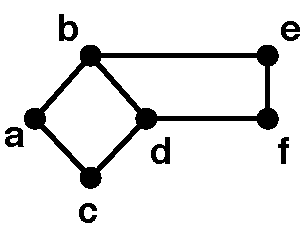
\includegraphics[scale=.75]{graph-contraction/contract-example1}
\vspace{-.2in}
\begin{eqnarray*}
V & = & \cset{\vname{a},\vname{b},\vname{c},\vname{d},\vname{e},\vname{f}}\\
E & = &
\{(\vname{a},\vname{b}),(\vname{b},\vname{a}),(\vname{b},\vname{d}),(\vname{b},\vname{e}),(\vname{e},\vname{b}),(\vname{d},\vname{b}),(\vname{d},\vname{f}),(\vname{a},\vname{c}),
\\
& & ~~(\vname{c},\vname{a}),(\vname{c},\vname{d}),(\vname{d},\vname{c}),(\vname{d},\vname{f}),(\vname{f},\vname{d}),(\vname{e},\vname{f}),(\vname{f},\vname{e})\}
\end{eqnarray*}
\end{center}
\end{example}

\begin{figure}
\begin{algorithm}[Counting Components using Graph Contraction]~
\label{alg:gc::cc}
\begin{lstlisting}[numbers=left]
countComponents $(G = (V,E))$ = 
  if $|E| = 0$ then $
    |V|$
  else 
    let 
      $(V',P)$ = starPartition $(V,E)$ @\label{line:gc::cc::partition}@
      $E'$ = $\csetf{(\cget{P}{u},\cget{P}{v}) : (u,v) \in E}{\cget{P}{u} \neq \cget{P}{v}}$ @\label{line:gc::cc::edges}@
    in
      countComponents $(V',E')$
    end
\end{lstlisting}
\end{algorithm}
\end{figure}


\algref{gc::cc} illustrates a  graph-contraction algorithm for determining
the number of connected components in a graph.
%
Each contraction on \lineref{gc::cc::partition} returns the set of
(centers) super-vertices $V'$ and a table $P$ mapping every $v \in V$
to a $v' \in V'$.
%
The set $V'$ defines the super-vertices of the quotient graph.
%
\lineref{gc::cc::edges} completes the computation of the quotient graph.
\begin{itemize}
\item it computes the edges of the quotient graph by 
routing the end points of each edge to the corresponding
super-vertices in $V'$, which is specified by the table $P$;
%
\item it  removes all self edges via the  filter $\cget{P}{u}
\neq \cget{P}{v}$.
%
\end{itemize}
%
Having computed the quotient graph, the algorithm recursively solves
the problem on it.
%
Recursion bottoms out when the graph contains no edges, in which case,
each component has been contracted down
to a singleton vertex, and thus the number of vertices in the
contracted graph is equal to the number of components in the input graph.

\begin{example}
The values of $V'$, $P$, and $E'$ after each round of the 
contraction shown in \exref{gc::contract-example}.
\[
\begin{array}{crcl}
  & V' & = & \cset{\vname{a},\vname{d},\vname{ef}}\\
\mbox{round } 1 & P' & = & 
 \cset{\vname{a} \mapsto \vname{a}, 
       \vname{b} \mapsto \vname{a}, 
       \vname{c} \mapsto \vname{a}, 
       \vname{d} \mapsto \vname{d}, 
       \vname{e} \mapsto \vname{e}, 
       \vname{f} \mapsto \vname{e}}\\
  & E' & = & \cset{(\vname{a},\vname{e}),
               (\vname{e},\vname{a}),
               (\vname{a},\vname{d}),
               (\vname{d},\vname{a}),
               (\vname{d},\vname{e}),
               (\vname{e},\vname{d})}\\[.1in]
  & V' & = & \cset{\vname{a},\vname{e}}\\
\mbox{round } 2 & P' & = & 
 \cset{\vname{a} \mapsto \vname{a}, 
       \vname{d} \mapsto \vname{abcd}, 
       \vname{e} \mapsto \vname{e}}\\
  & E' & = & \cset{(\vname{a},\vname{e}),
               (\vname{e},\vname{a})}\\[.1in]
  & V' & = & \cset{\vname{a}}\\
\mbox{round } 3 & P' & = & 
 \cset{\vname{a} \mapsto \vname{a}, 
       \vname{e} \mapsto \vname{a}}\\
  & E' & = & \cset{}
\end{array}
\]
\end{example}


Our previous algorithm just counted the number of components. 
%
We can modify the algorithm slightly to compute the components
themselves instead of returning their count. 
%
To this end, we are going to construct the mapping from vertices to
their components recursively. This is possible because we can obtain
the mapping by composing the mapping from vertices to their
super-vertices and the mapping from super-vertices to their
components, which we obtain recursively. \algref{gc::nc} shows the
algorithm.

\begin{figure}
\begin{algorithm}[Contraction-based graph connectivity]
~
\label{alg:gc::nc}
\begin{lstlisting}[numbers=left]
connectedComponents $(G = (V,E)) = $
  if $|E| = 0$ then 
    $(V, \cset{v \mapsto v : v \in V})$
  else 
    let 
      $(V',P) =$ starPartition $(V,E)$
      $E' = \csetf{(\cget{P}{u},\cget{P}{v}) : (u,v) \in E}{\cget{P}{u} \neq \cget{P}{v}}$ 
      $(V'',C) =$ connectedComponents $(V',E')$
    in
      $(V'', \cset{v \mapsto C[s] : (v \mapsto s) \in P})$ @\label{line:gc::nc::back}@
  end
\end{lstlisting}
% old code : \cset{v \mapsto \cget{P'}{\cget{P}{v}} : v \in V}
\end{algorithm}
\end{figure}

\begin{example}~
\label{ex:concomp}
\vspace{-.2in}
\begin{center}
$\cname{connectedComponents}\left(\raisebox{-.5in}{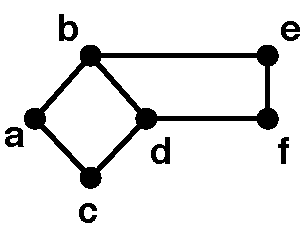
\includegraphics[scale=.6]{graph-contraction/contract-example1}}\right)$
\end{center}
might return:
\begin{eqnarray*}
(\cset{\vname{a}}, ~\cset{\vname{a} \mapsto \vname{a}, 
                          \vname{b} \mapsto \vname{a}, 
                          \vname{c} \mapsto \vname{a}, 
                          \vname{d} \mapsto \vname{a}, 
                          \vname{e} \mapsto \vname{a}, 
                          \vname{f} \mapsto \vname{a}})
\end{eqnarray*}
since there is a single component and all vertices will map to that
component label.  In this case \vname{a} was picked as the
representative, but any of the initial vertices is a valid
representative, in which case all vertices would map to it.
\end{example}

The only differences from \cname{countComponents} are a modification
to the base case, and the extra line (\lineref{gc::nc::back}) after
the recursive call.  In the base case instead of returning the size of
$V$ returns all vertices in $V$ along with a mapping from each one to
itself.  This is a valid answer since if there are no edges each
vertex is its own component.  In the inductive case, when returning
from the recursion, \lineref{gc::nc::back} updates the mapping $P$
from vertices to super-vertices by looking up the component that the
super-vertex belongs to, which is given by $C$.  This simply involves
the look up $C[s]$ for every $(v \mapsto s) \in P$.  Note that if you
view a mapping as a function, then this is equivalent to function
composition, i.e., $C \circ P$.

\begin{example}
  Consider our example graph (\exref{concomp}), and assume that
  \cname{starPartition} returns:
\begin{eqnarray*}
V' & = & \cset{\vname{a},\vname{d},\vname{e}}\\
P & = & 
 \cset{\vname{a} \mapsto \vname{a}, \vname{b} \mapsto \vname{a}, 
       \vname{c} \mapsto \vname{a}, \vname{d} \mapsto \vname{d}, 
       \vname{e} \mapsto \vname{e}, \vname{f} \mapsto \vname{e}}.
\end{eqnarray*}
%
This pairing corresponds to the case where $a$, $d$ and $e$ are chosen
an centers.
%
Since the graph is connected, the recursive call to
\cname{connectedComponents}$(V',E')$ will map all vertices in $V'$ to
the same vertex.  Lets say this vertex is \vname{a} giving:
\begin{eqnarray*}
V'' & = & \cset{\vname{a}}\\
P' & = & \cset{\vname{a} \mapsto \vname{a}, \vname{d} \mapsto \vname{a}, \vname{e} \mapsto \vname{a}}~.
\end{eqnarray*}
%
Now $\cset{v \mapsto P'[s] : (v \mapsto s) \in P}$ will for each
vertex-super-vertex pair in $P$, look up what that super-vertex got
mapped to in the recursive call.  For example, vertex \vname{f} maps
to vertex \vname{e} in $P$ so we look up \vname{e} in $P'$, which
gives us \vname{a} so we know that \vname{f} is in the component
\vname{a}.  Overall the result is:
%
\[\cset{\vname{a} \mapsto \vname{a}, 
                          \vname{b} \mapsto \vname{a}, 
                          \vname{c} \mapsto \vname{a}, 
                          \vname{d} \mapsto \vname{a}, 
                          \vname{e} \mapsto \vname{a}, 
                          \vname{f} \mapsto \vname{a}}\;.\]
\end{example}


\paragraph{Cost of connected-components algorithms.}


\begin{remark}
  In general the graph contraction techniques does not specify how to
  partition the graph.  In this chapter, we
  considered two techniques for graph partitioning.  Depending on the problem,
  other techniques can be used.  For graph contraction to be
  applicable to a problem, however, it is important that the quotient graph satisfy certain properties.  For example,
  when solving graph connectivity with the algorithms described here,
  we have to be careful that the graph partition maintains connectivity:
  a subgraph should be connected in the quotient graph, if and only if
  it was connected in the input graph.  To ensure this,
  we will need to use a graph-partition algorithm that ensures that each
  part is connected in the input graph.  For example, the pictures
  below illustrate two graph partitions. The first graph partition
  maintains connectivity,  the second one does not.

\begin{center}
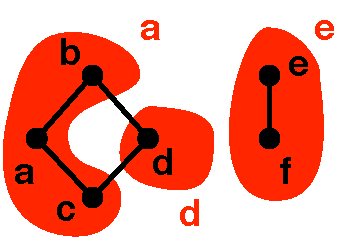
\includegraphics[width=1.6in]{graph-contraction/partition-example1}
\hspace{1in}
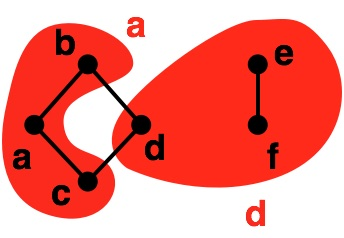
\includegraphics[width=1.7in]{graph-contraction/partition-example2}

\end{center}
The partitioning on the left is appropriate for graph contraction since
each partition is connected.    The partition on the right is not
since $\cname{d}$ is not connected to $\cname{e}$ and $\cname{f}$.
\end{remark}



\section{Forest Contraction and Tree Contraction}
Suppose that we want to contract a forest of trees instead of  a
general graph as we considered thus far.
% 
Since forests are graphs, we can use the same \cname{starPartition}
algorithm to contract the forest.
%
Since a forest of $n$ vertices has at most $n-1$ edges, we obtain a
better work bound,  because the number of edges
decrease geometrically (in expectation) in each round, as do the
number of vertices.  
%
The overall expected work is therefore a
geometric sum of the form: 
%
\[
\expct{W(n,m)} = \sum_{i=0}^{\infty} \left(\frac{3}{4}\right)^i kn =
O(n),
\] 
%
instead of $O(m \log n)$ for
general graphs.  The span is not affected.
%
The same bound applies if the forest is connected, and thus is a tree.

For a graph $G = (V,E)$ consider a subset of edges $F \subset E$ that
forms a forest (i.e., has no cycles).  Such a set of edges partitions
the graph $G$, where parts are defined as the subgraphs induced by
the trees in $F$.
%
\begin{question}
How can we perform graph contraction by using trees for partitioning?
\end{question}
%
We can thus contract a graph by identifying a forest $F$, and then use
\cname{connectedComponents} $(V,T)$, which does
linear work as explained above, instead of our \cname{starPartition}
routine.  
%
This corresponds to \defn{tree partitioning} instead of star or edge
partitioning, which are special kinds of trees.
%
We will use this idea in an algorithm for Minimum Spanning
Trees described in \chref{mst}.

\begin{example}
A graph and a subset of the edges $F$ (highligted) consisting of
three disjoint trees illustrated in the middle diagram.  Each tree
induces a part in the original graph (red blobs). 
 
\begin{center}
  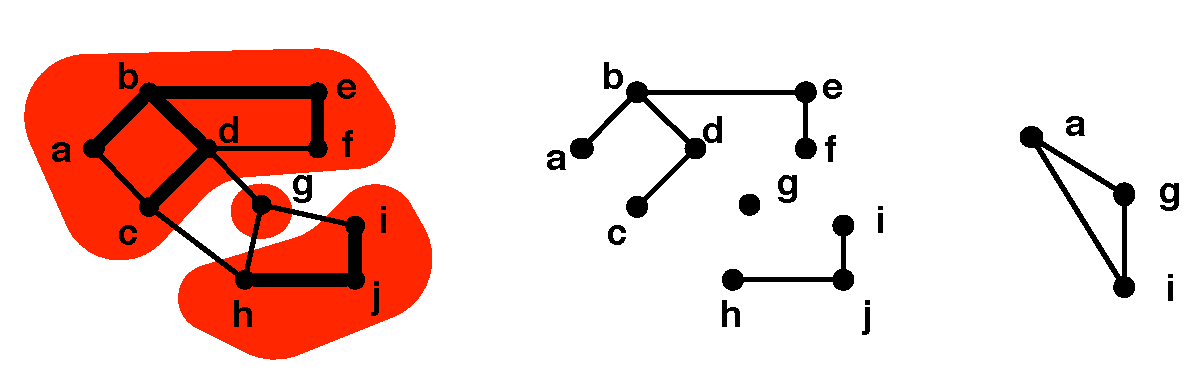
\includegraphics[scale=.7]{graph-contraction/tree-contract-example}
\end{center}
If we run \cname{connectedComponents} on $F$, then are left with the desired partitioning with
super-vertices $\cset{\vname{a},\vname{g},\vname{i}}$ and the mapping:
%
\[
\cset{\vname{a}\mapsto\vname{a},\vname{b}\mapsto\vname{a},\vname{c}\mapsto\vname{a},\vname{d}\mapsto\vname{a},\vname{e}\mapsto\vname{a},\vname{f}\mapsto\vname{a},
  \vname{g}\mapsto\vname{g},
  \vname{h}\mapsto\vname{i},\vname{i}\mapsto\vname{u},\vname{j}\mapsto\vname{i}}.
\]

Using this partition, we can compute a quotient graph in the usual
way by re-routing edges to the super-vertices.  The resulting quotient graph is 
illustrated on the right.

\end{example}


\begin{comment}
\section{Spanning Trees and Forests}


A \emph{spanning tree} of an undirected connected graph $G = (V,E)$ is
a tree $T = (V,E')$ where $E' \subseteq E$.  A \emph{spanning forest}
of a graph $G = (V,E)$ is the union of spanning trees on its connected
components.  We are interested in the spanning forest problem, which
is to find a spanning forest for a given undirected graph (the
spanning tree is just the special case when the input graph is
connected).

It turns out that a spanning forest of a graph $G$ can be generated
from our connectivity algorithm.  In particular all we need to do is
keep track of all the edges that we use to hook, and return the union
of these edges.  We will see this in more detail as we cover minimum
spanning trees, our next topic.
\end{comment}

\section{Problems}

\begin{probl}{}
There are 18 subgraphs for a triangle consisting of three vertices
and three edges connecting them, including the empty graph and the graph
itself.    List them all.
\end{probl}


\begin{probl}{}
In star contraction, what is the probability that a vertex with degree
$d$ is removed.
\end{probl}


\begin{probl}{}
Find an example graph, where star-based graph contraction removes a
small number of edges on each round.
\end{probl}

% Solution: a graph consisting of small stars that are connected with
% many edges. The star will be removed but all the cross edges between
% them will remain.  Must repeat this recursively to find the right
% structure.

\begin{probl}{}
Describe how to construct a graph that exhibits the worst-case
behavior for \thmref{gc::star-contraction-cost}.
\end{probl}

\begin{probl}{}
Is the star contraction algorithm work-optimal for a dense graph with
$\Omega(n^2)$ edges? Prove or disprove.
\end{probl}

 
}
\flushchapter
